\chapter{Ongoing work and future directions}

There is still a lot that can be done to improve the detector in various fronts, this chapter suggests possible paths to build upon the work included in this document.

\section{Odd features in measured spectra}

Figure \ref{fig:NIM_odd_features} summarizes some odd features found while measuring spectra with the NIM modules, some of them can also be found in the spectra obtained with the Rohde\&Schwarz oscilloscope. The high number of counts above the photopeak and the oddly shaped photopeaks (``shoulders'' on the high energy side, also discussed in \cite{peak_shoulders}) could make for an interesting study.

\section{Geant4 simulation}

\subsection{Adding LYSO radioactivity}

As mentioned in Section \ref{sec:self_radiation} and subsection \ref{sec:simulated_spectra}, LYSO:Ce crystals have self radiation, this feature has not yet been added to the simulation, and would be an interesting exercise to showcase how Geant4 can recreate this type of physical process.

\subsection{Improving data recollection}

All the results included in Chapter \ref{chap:G4_simulations} are extracted in \texttt{stepAction.cc}, by checking the current volume of the particle and extracting data accordingly. This approach, however, is very inefficient, since it performs multiple operations for every step of every particle created in the simulation. In order to improve this one could make use of the \texttt{G4VSensitiveDetector} class, which calls the \texttt{ProcessHits} function once a particle enters the sensitive volume, in our case this volume could be the SiPM or scintillating material.

\section{Testing different scintillator sizes and materials}

The scintillator size can have great consequences on the resulting spectra and therefore energy resolution, as is showcased in subsections \ref{sec:simulated_spectra} and \ref{sec:collected_produced}, this opens up a great opportunity to explore the possibility of testing other crystal sizes, since up until now only the $4\times4\times22$ \unit{\mm\cubed} LYSO has been used to measure spectra. Some photos of available crystal sizes provided by Luxium are shown in Fig. \ref{fig:LYSO_crystals}. On the other hand, it could also be useful to try BGOs, these crystals are also sold for relatively low prices, this however tend to show better results at energy ranges above our use case.

\begin{figure}[H]
    \begin{subfigure}[t]{0.49\textwidth}
        \centering
        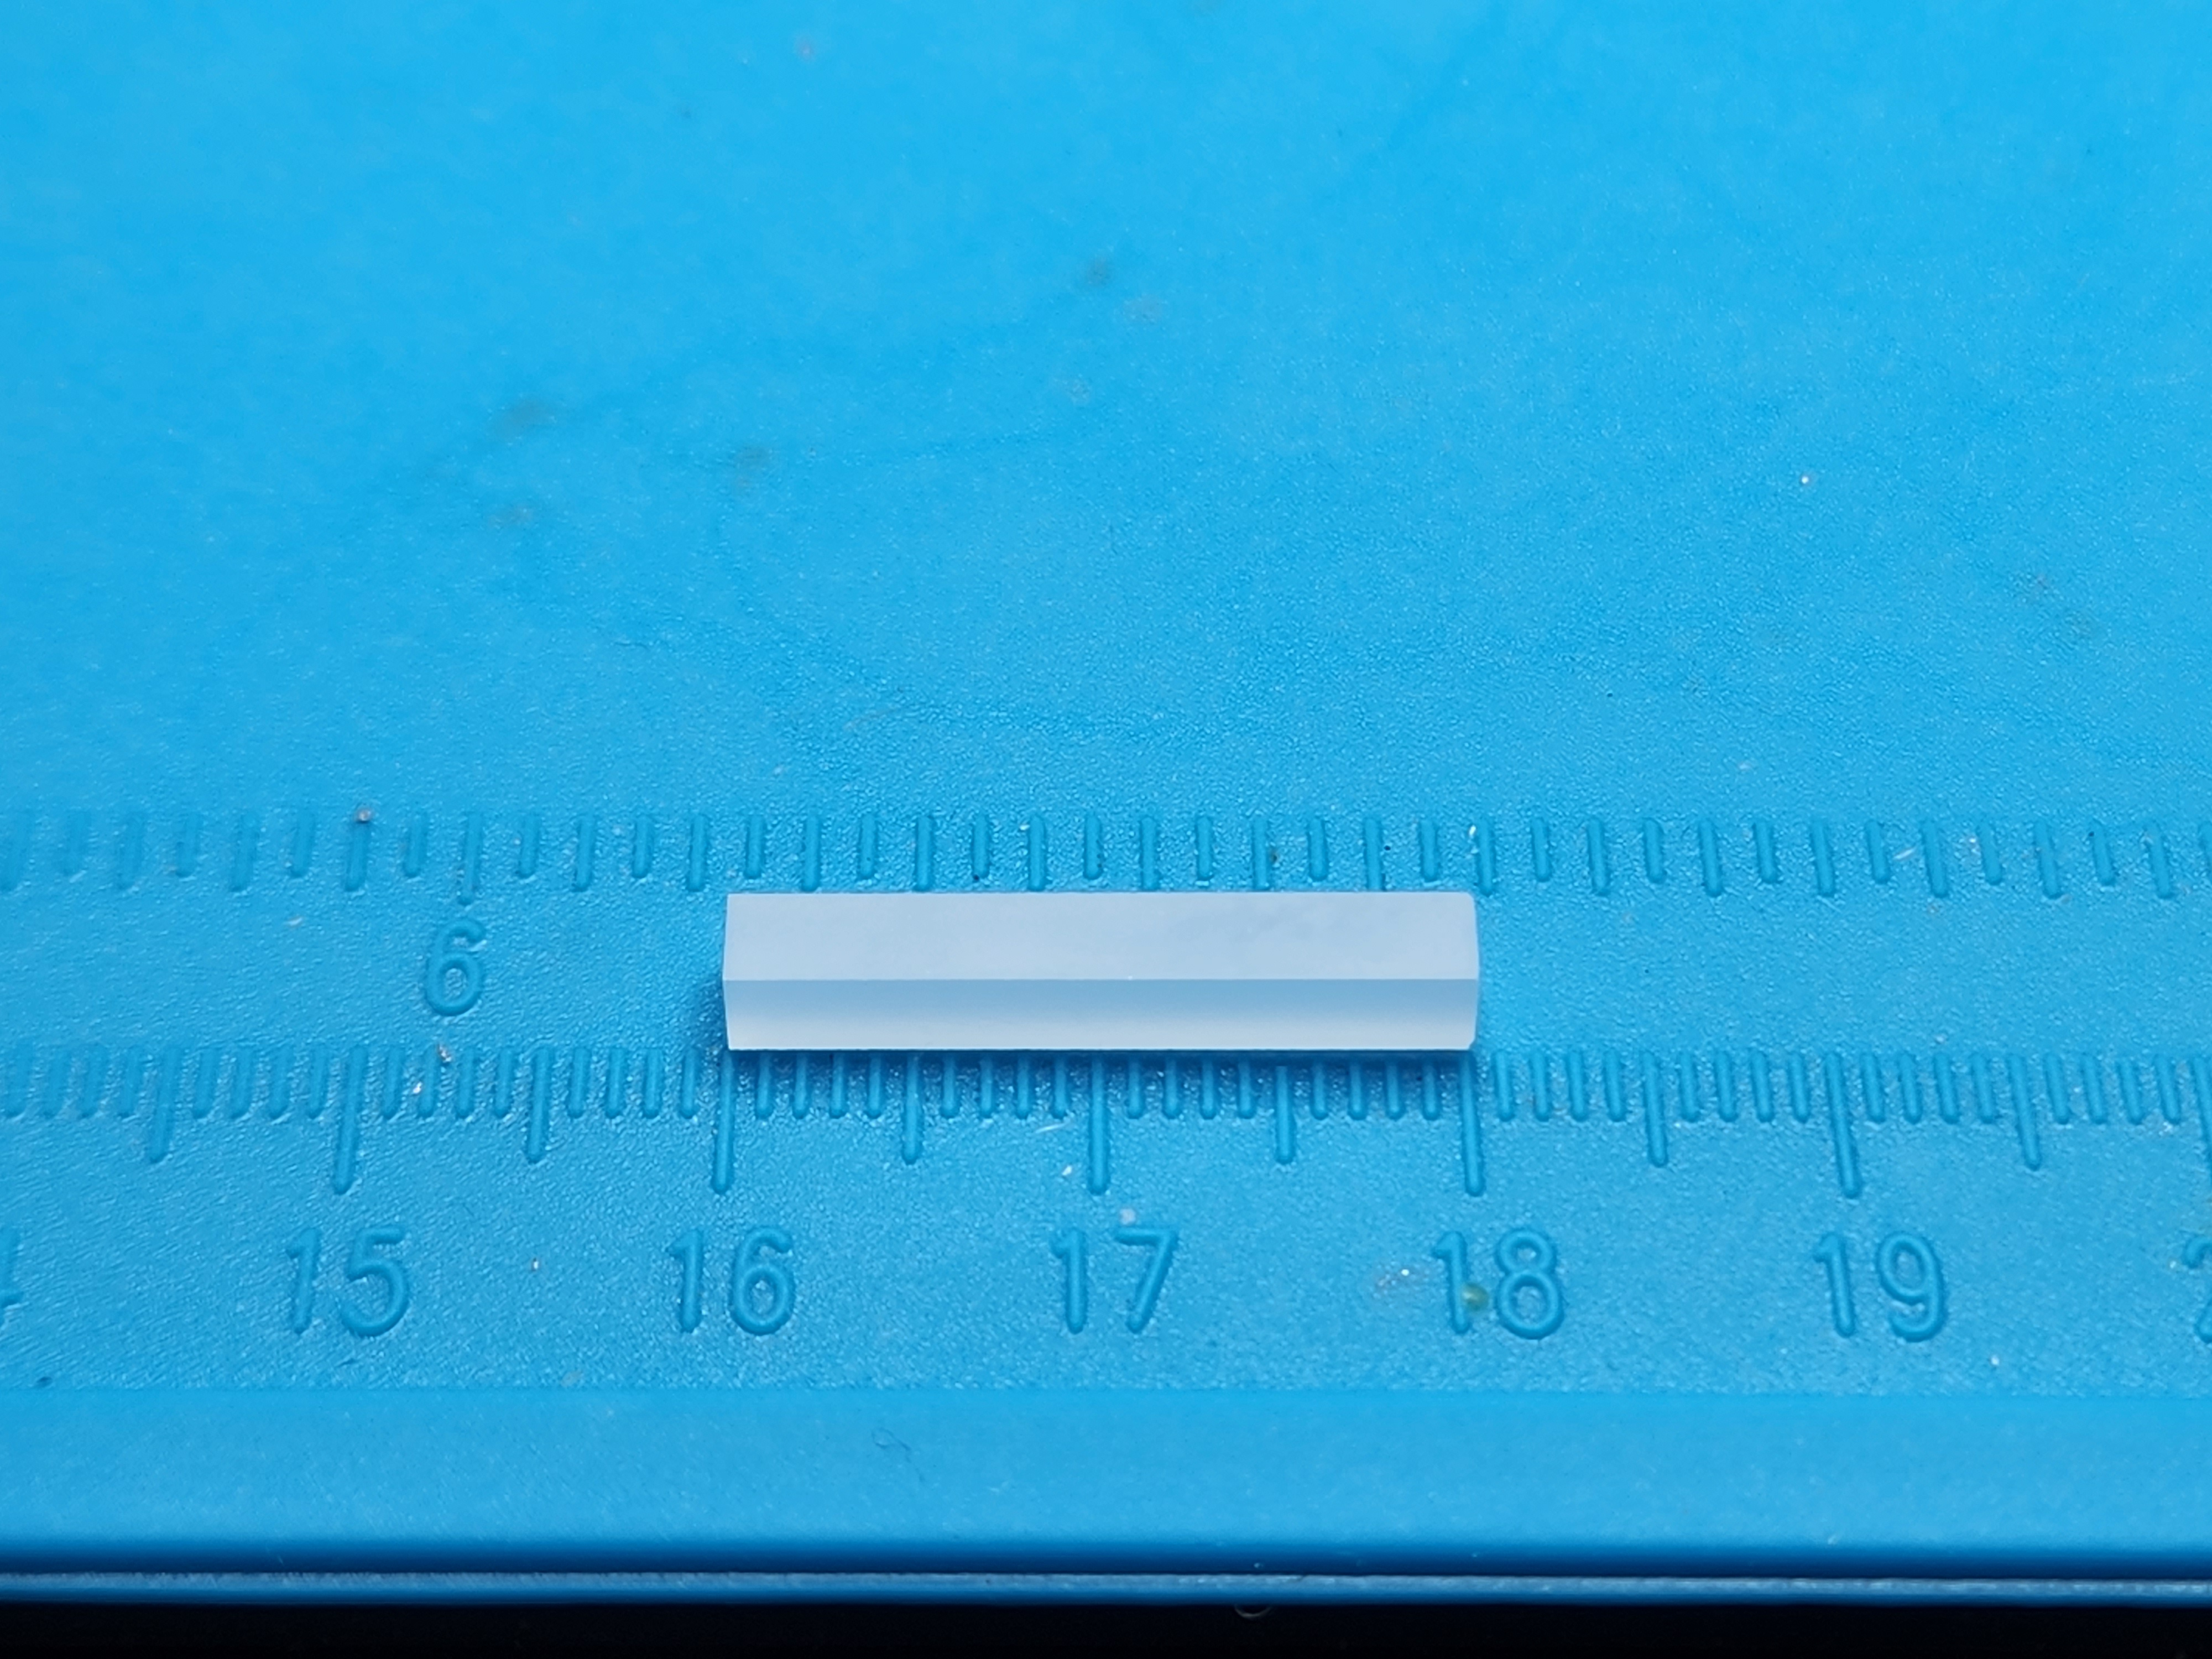
\includegraphics[width=.7\textwidth]{future/LYSO_crystals/LYSO_20_3_3.jpg}
    \end{subfigure}
    \begin{subfigure}[t]{0.49\textwidth}
        \centering
        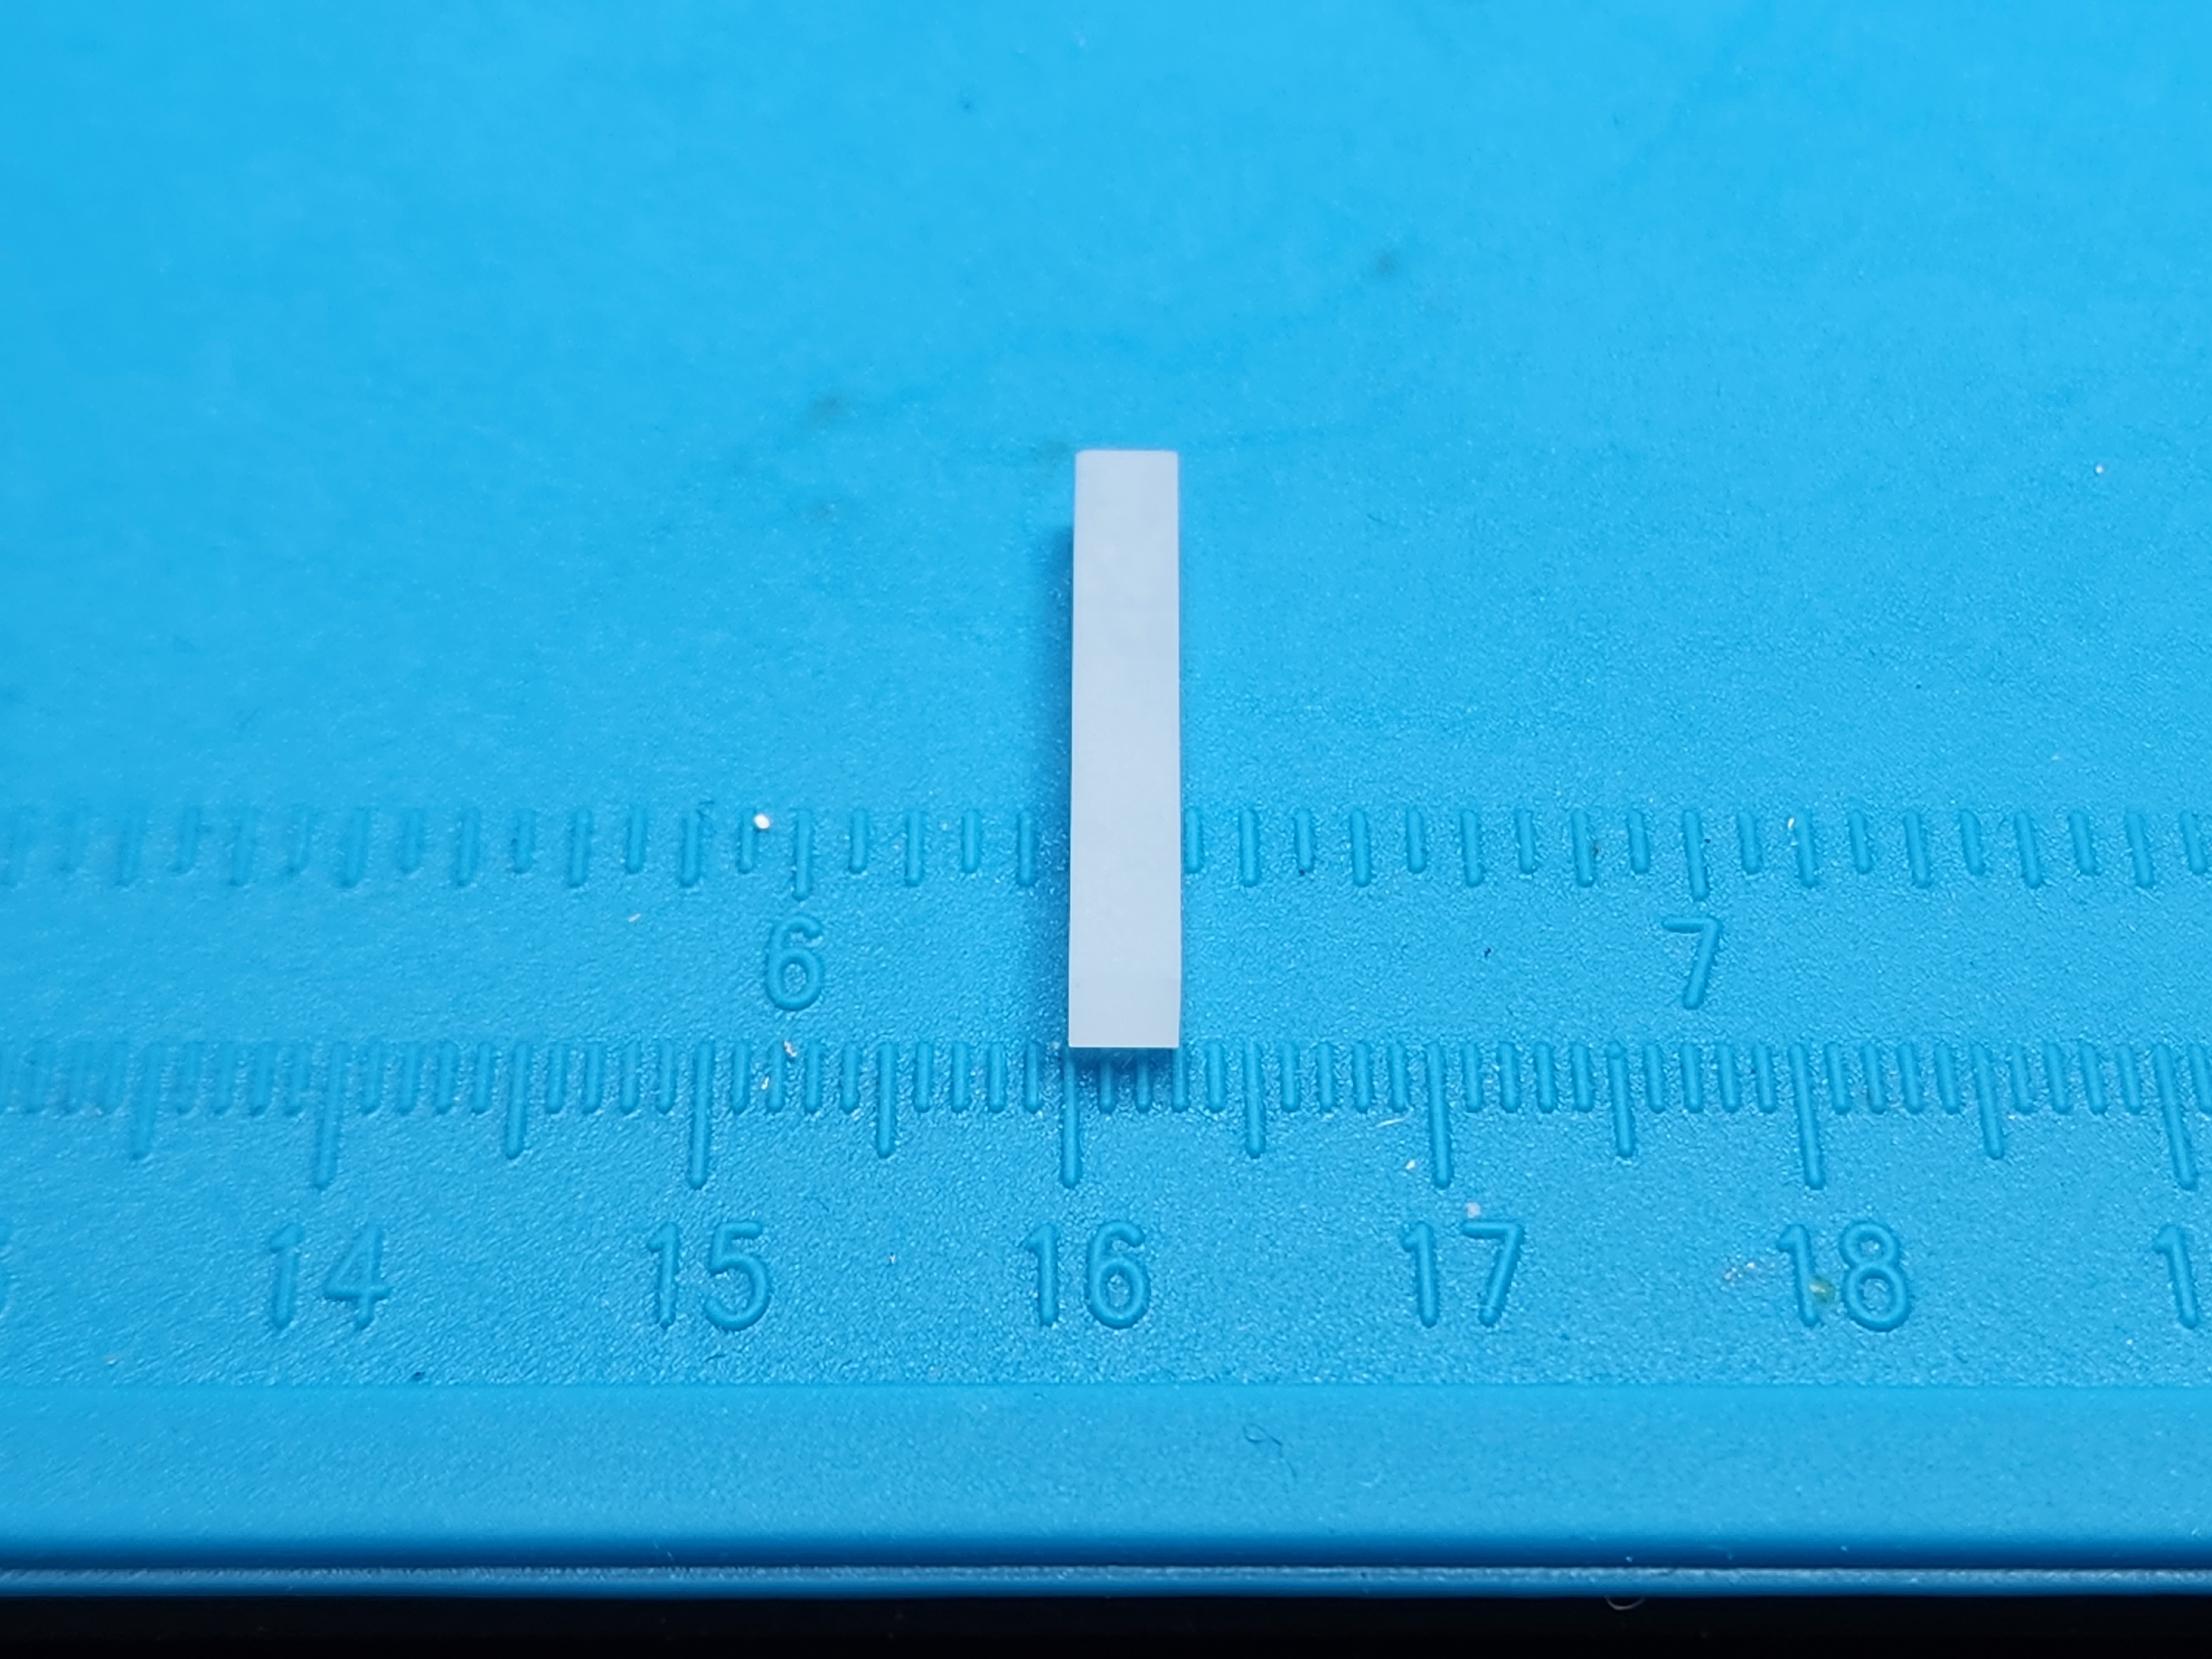
\includegraphics[width=.7\textwidth]{future/LYSO_crystals/LYSO_20_3_3_2.jpg}
    \end{subfigure}
    \medskip
    \begin{subfigure}[t]{0.49\textwidth}
        \centering
        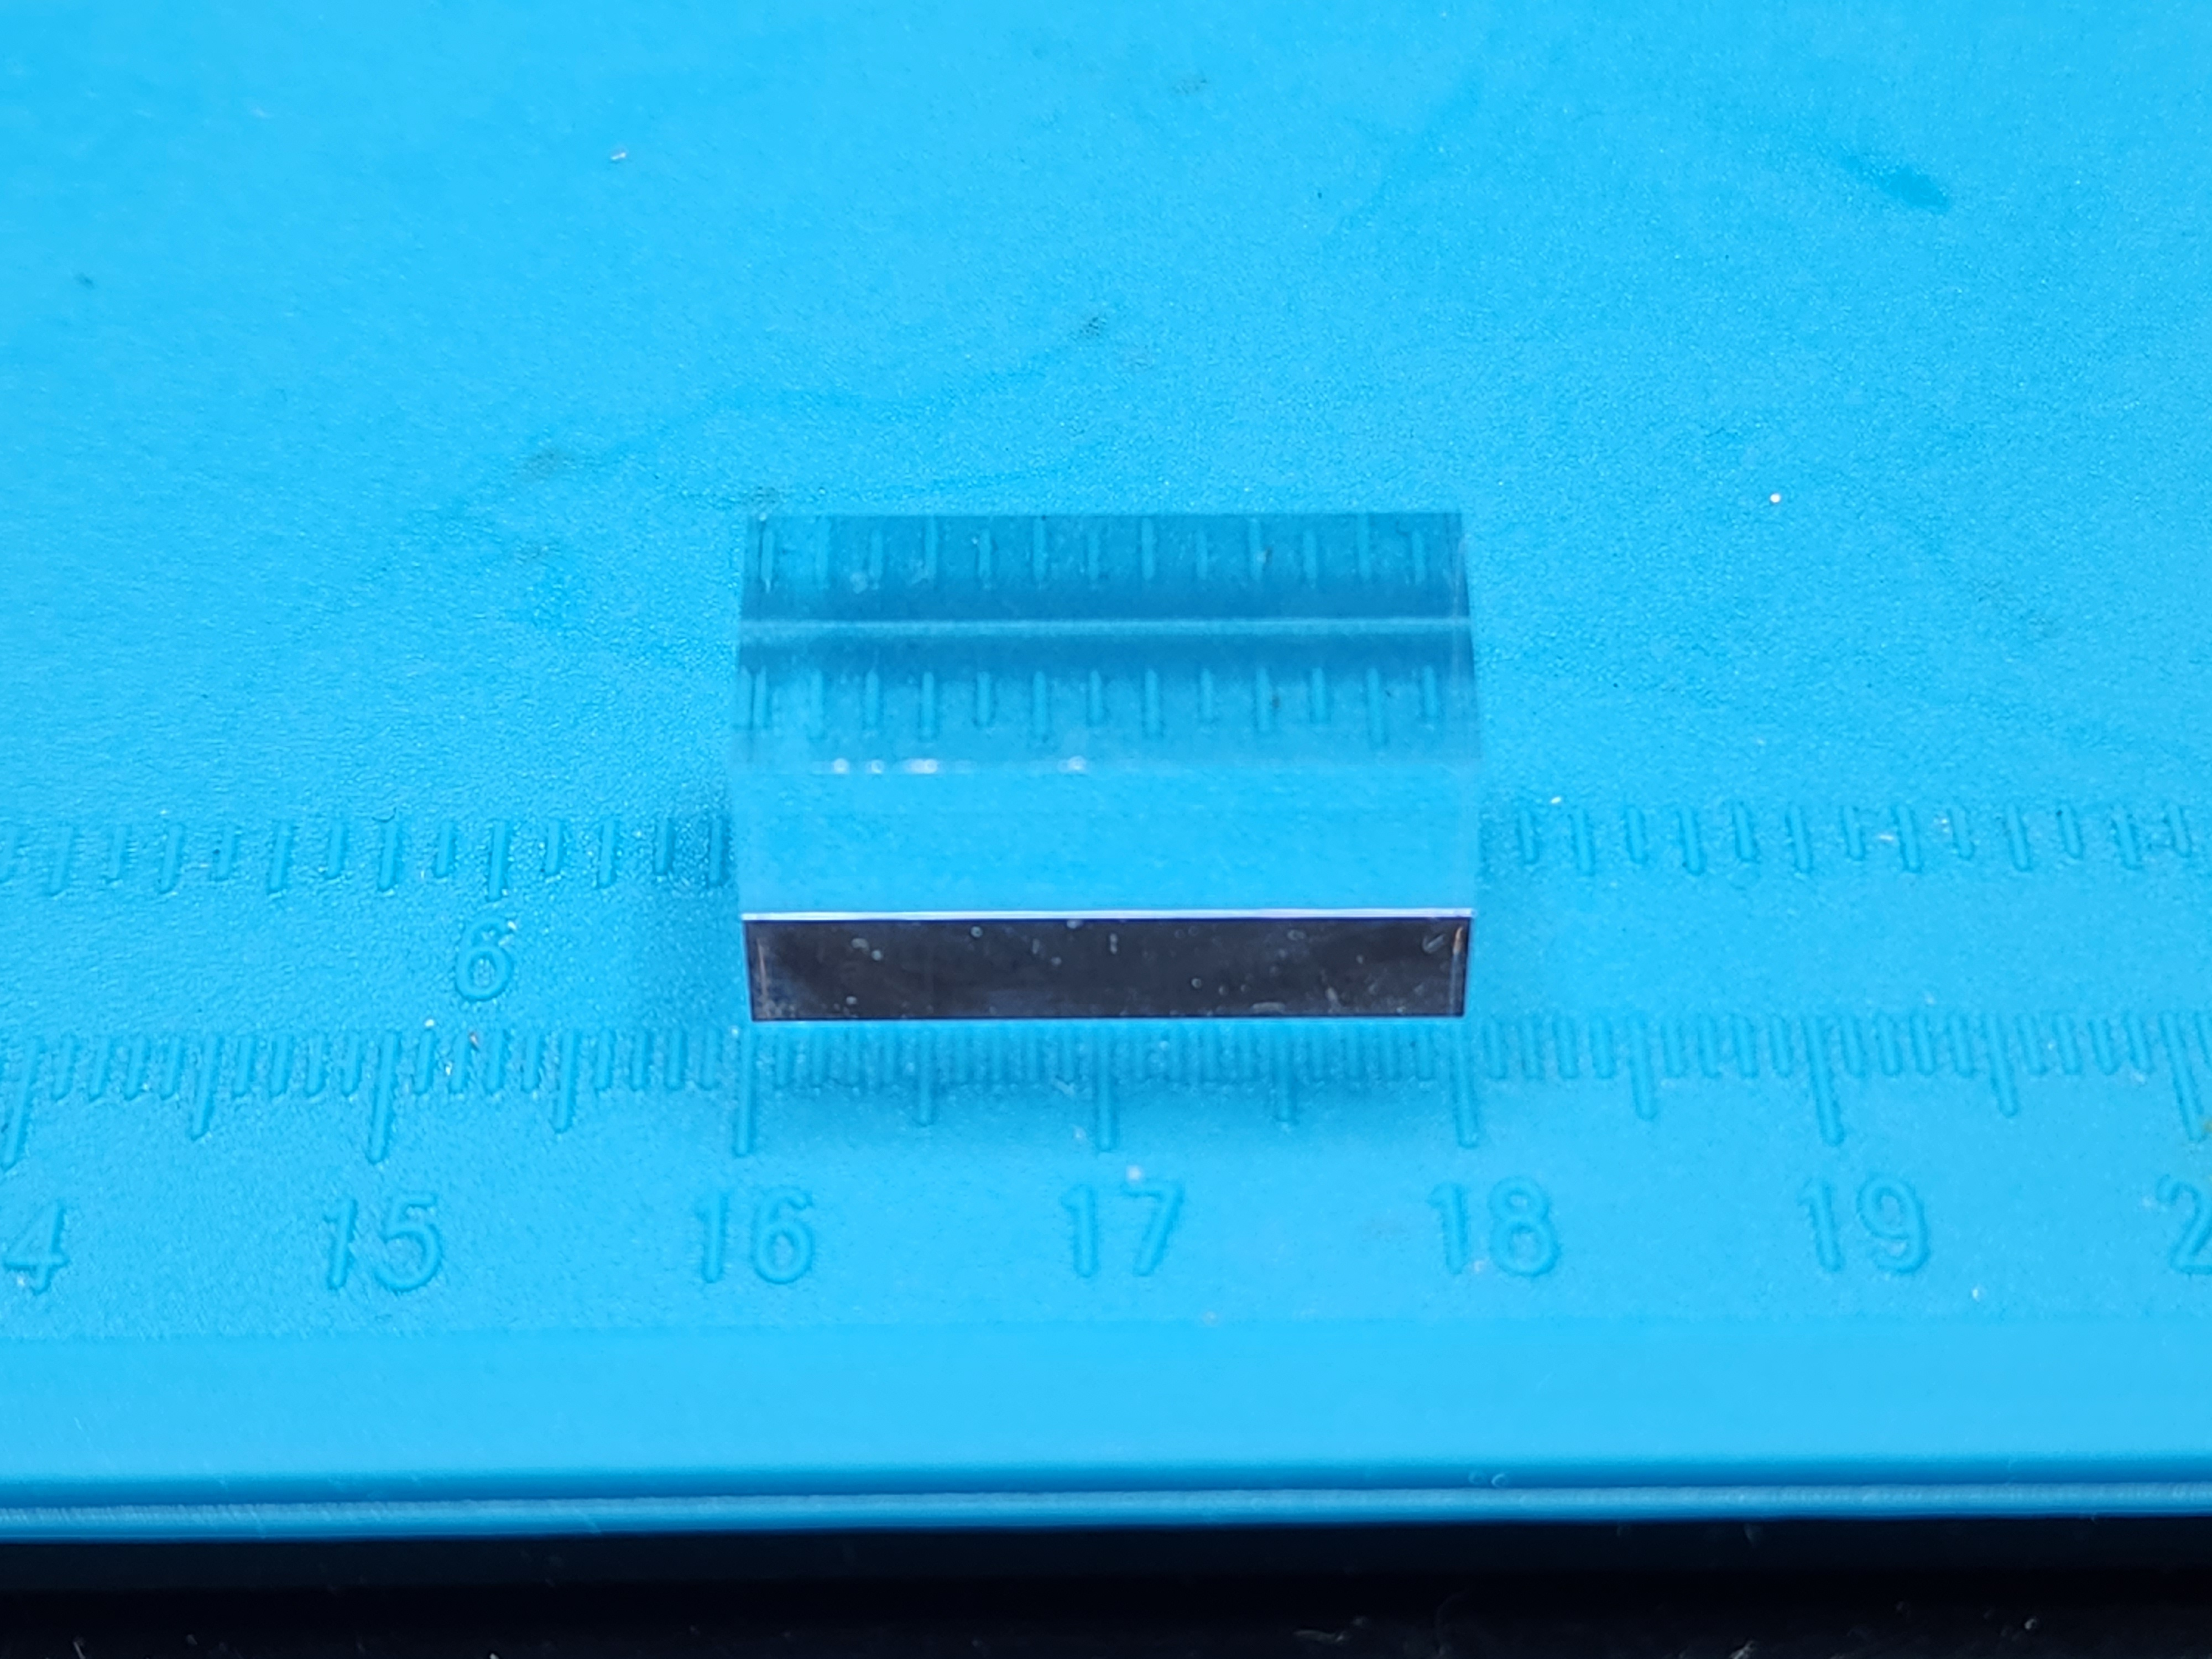
\includegraphics[width=.7\textwidth]{future/LYSO_crystals/LYSO_20_10_10.jpg}
    \end{subfigure}
    \begin{subfigure}[t]{0.49\textwidth}
        \centering
        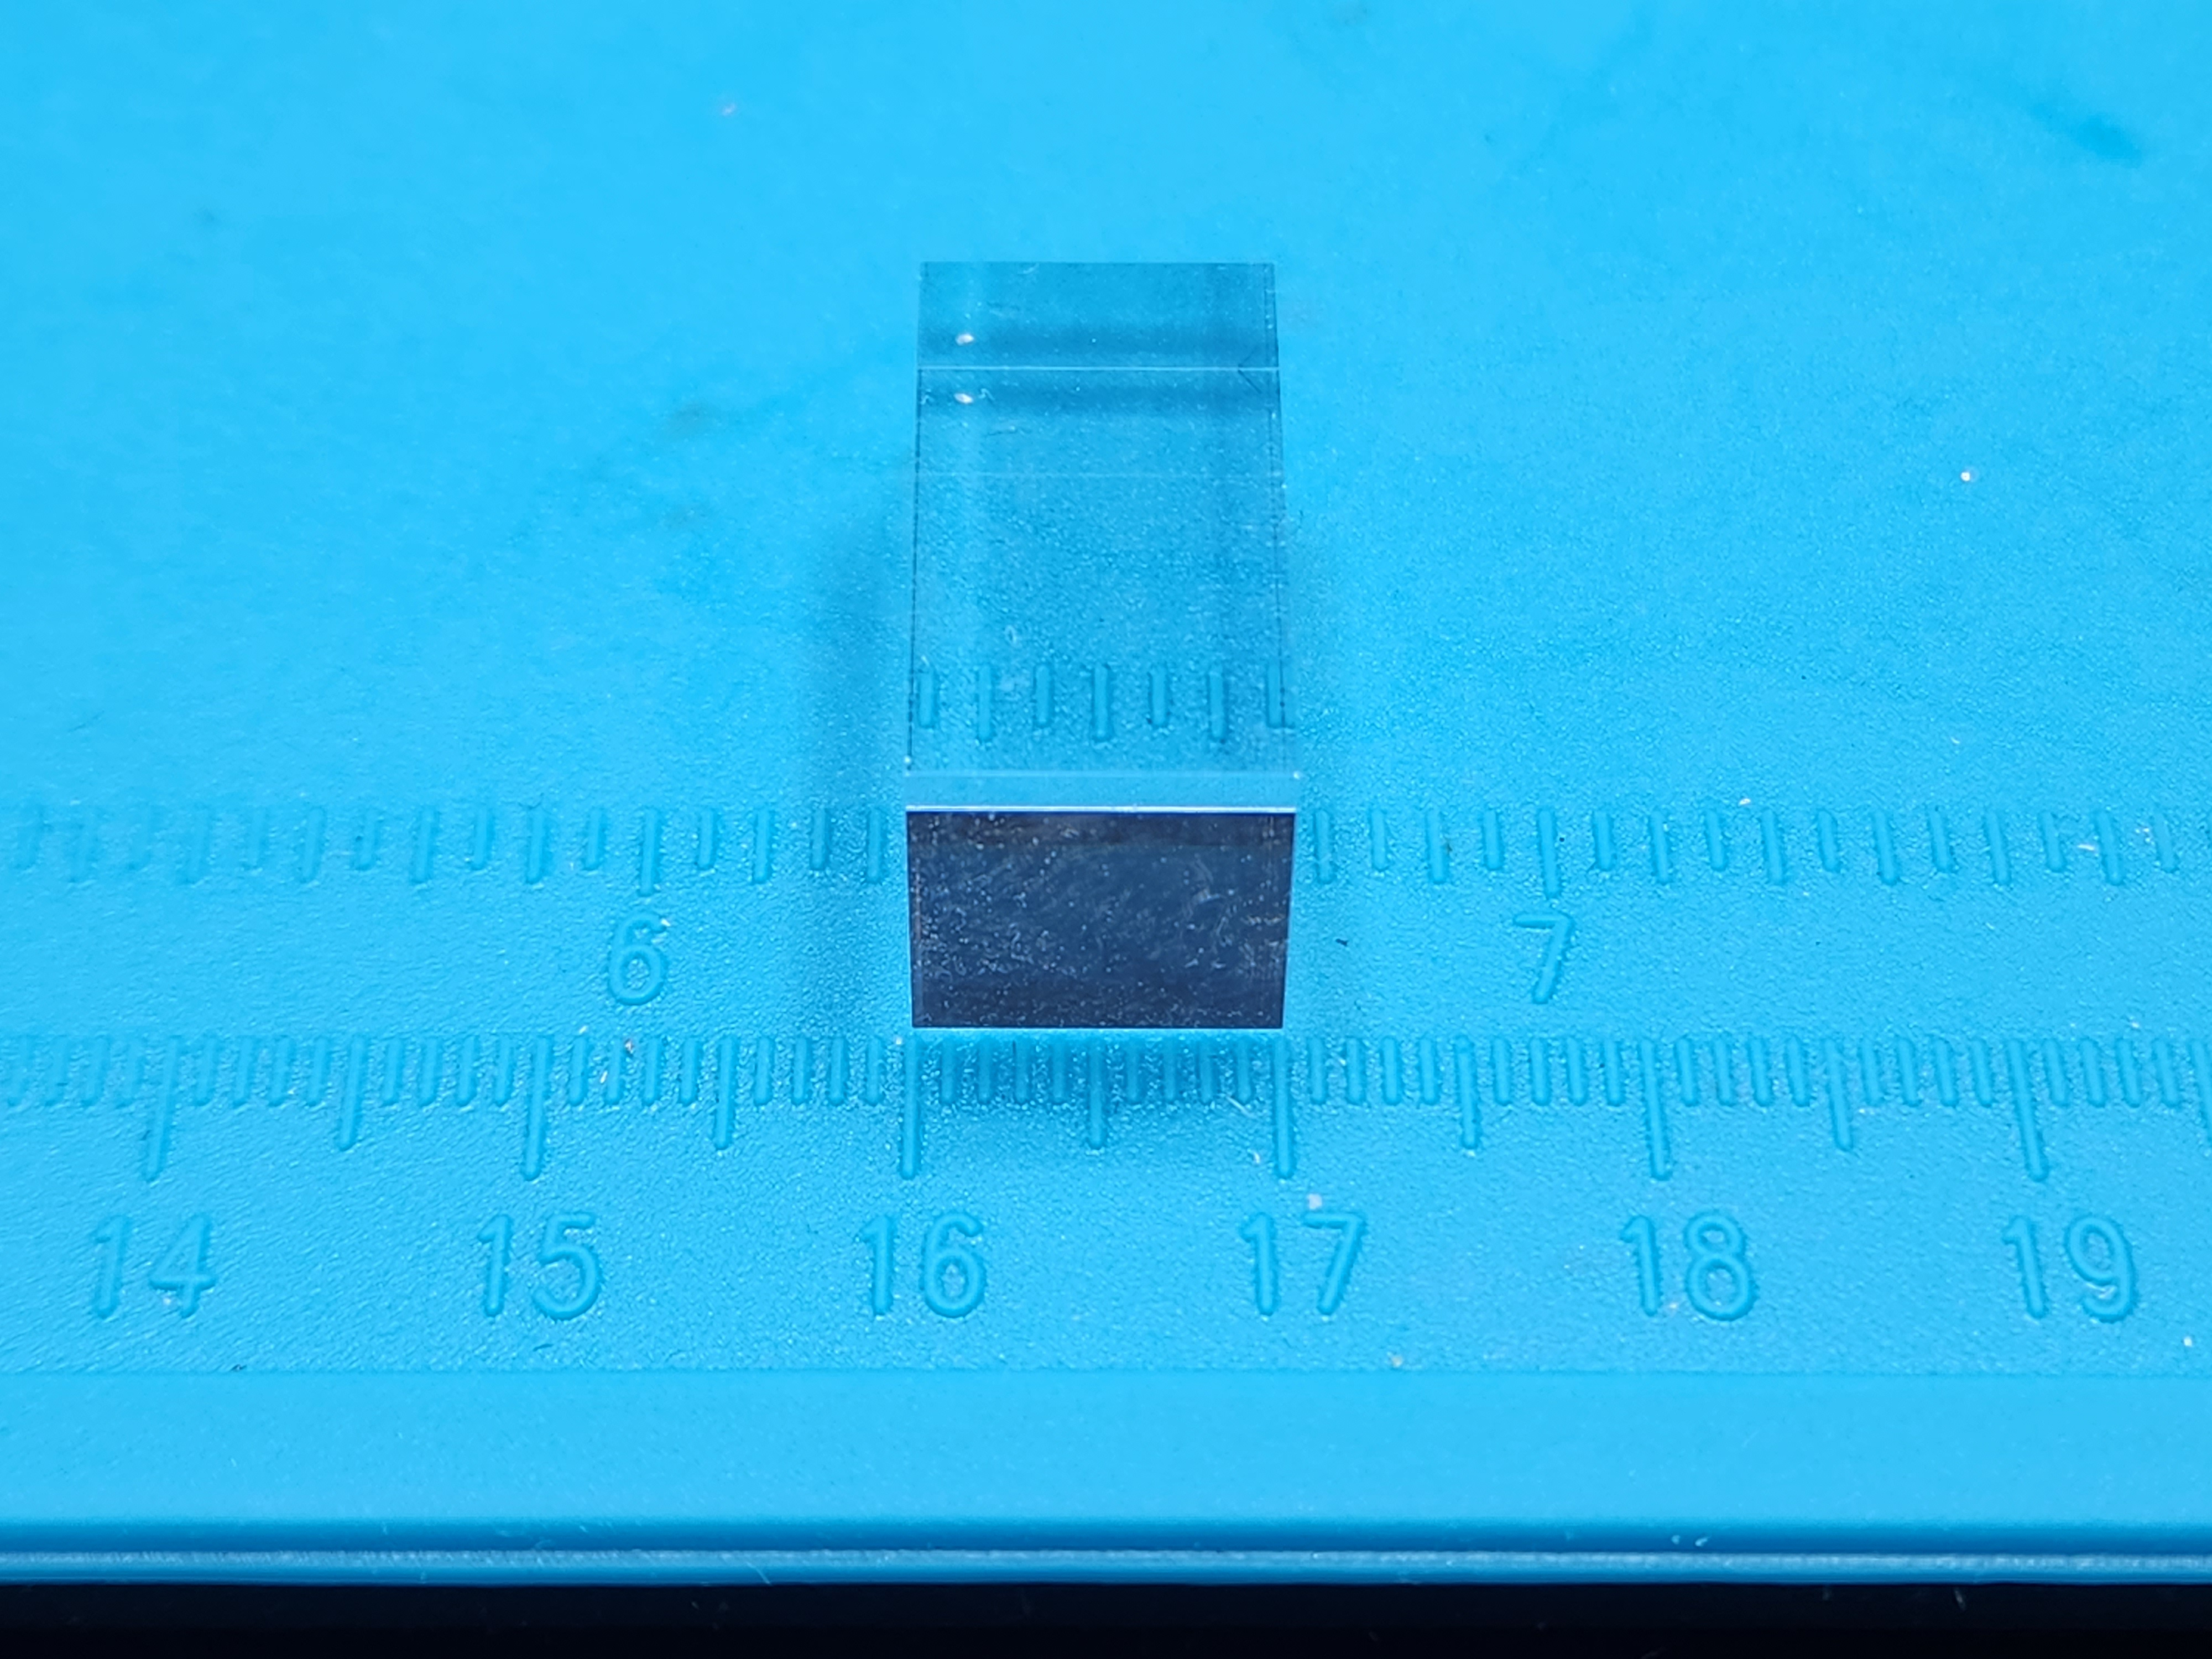
\includegraphics[width=.7\textwidth]{future/LYSO_crystals/LYSO_20_10_10_2.jpg}
    \end{subfigure}
    \medskip
    \begin{subfigure}[t]{\textwidth}
        \centering
        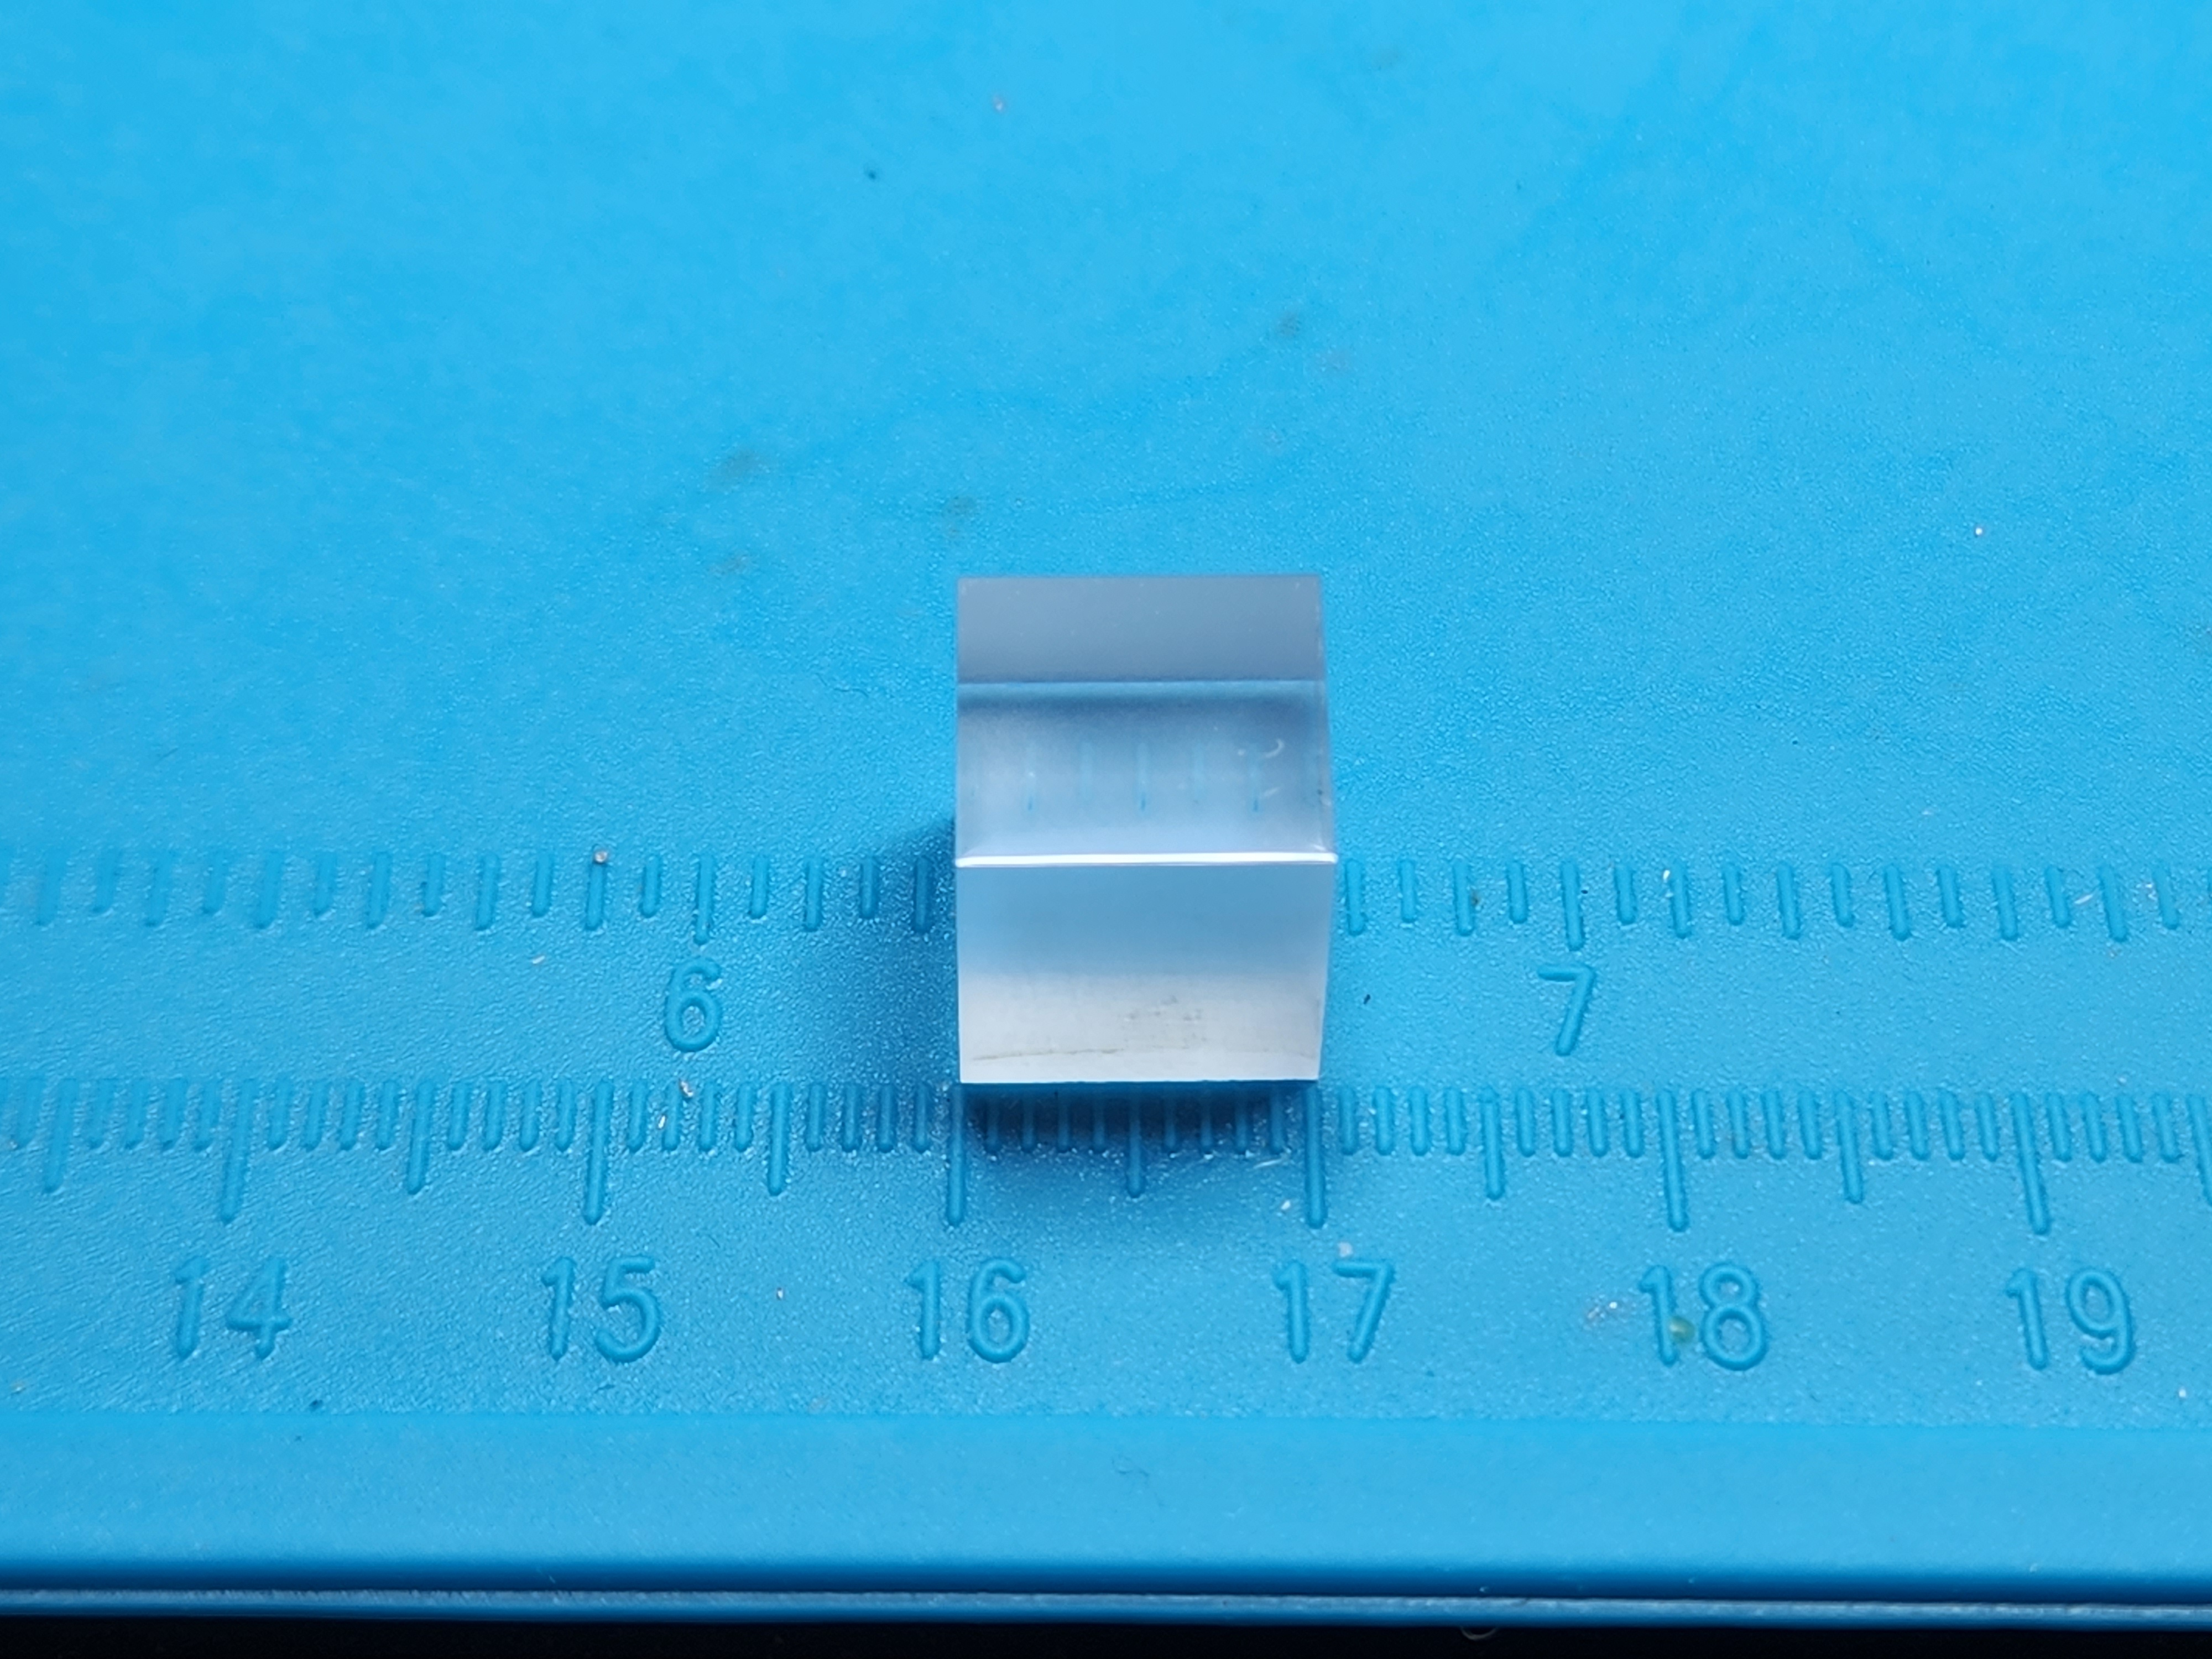
\includegraphics[width=.35\textwidth]{future/LYSO_crystals/LYSO_10_10_10.jpg}
    \end{subfigure}
    \caption{\label{fig:LYSO_crystals}Dimensions of LYSO crystals used to test the CosmicWatch response.}
\end{figure}

\section{Microcontroller}

\subsection{Code}

An interesting route yet to be explored is the use of the \texttt{C++} SDK, MicroPython could 

\the\textwidth